\chapter{Graphing}

The graphing component is reused in many places throughout the Corina desktop application.  The following description although based on the main graphing screen in Corina is largely applicable to all dialogs that include graphs (e.g.\ crossdating, indexing and reconciliation).  

The main method for graphing your tree-ring data is by choosing an option from the Graph menu.  Depending on the type of series you have open, the options available to you will be different.  For raw measurement series, you will just have the option to `Graph active series'.  This will give you a simple graph of the current series that you have open.  If you have a derived series open, then you may also choose `Graph component series' which will plot all the series that go to create this series, or 'Graph all series' which graphs all the component series as well as the current series.

\section{Controlling graphs}

When newly created graphs are plotted according to the scale on the axes.  A feature of Corina graphs though is that they can be manipulated directly on the screen.  Both dendrochronology was computerized, dendrochronologists would plot rings manually on to graph paper.  These paper graphs were then placed on lightboxes and moved around to enable comparisons.  The graph function in Corina emulates this behaviour allowing users to click and drag graphs around to test for visual matches.

Figure \ref{fig:graph} shows an example graph dialog.  The mouse is hovering of the blue measurement series at relative year 1040 illustrating Corina's highlighting and guide line capabilities.  A feature not shown in this screenshot is the illustration of sapwood rings.  When sapwood rings are present the corresponding years on the chart are denoted via a heavier line.

\begin{figure}[hbtp]
  \centering
    
\includegraphics[width=0.6\textwidth]{Images/graph.png}
    \caption{An example graph window containing two undated series of the same sample on a semi-log graph.  Note the legend is visible with the options for adding or removing series.}
    \label{fig:graph}
\end{figure}


The layout of graphs can be changed using both the toolbar buttons and menu options.  The type of graph can be changed between a standard line graph, a semi-log graph and a toothed graph using the radio buttons.  The remaining buttons are as follows:

\begin{center}
\begin{tabular*}{0.8\textwidth}[h]{lp{10cm}}
 
\includegraphics[width=4mm]{../src/edu/cornell/dendro/corina_resources/Icons/22x22/haxiszoomin.png} & Zoom in on the horizontal axis \\
 
\includegraphics[width=4mm]{../src/edu/cornell/dendro/corina_resources/Icons/22x22/haxiszoomout.png} & Zoom out on the horizontal axis \\
 
\includegraphics[width=4mm]{../src/edu/cornell/dendro/corina_resources/Icons/22x22/vaxiszoomin.png} & Zoom in on the vertical axis \\
 
\includegraphics[width=4mm]{../src/edu/cornell/dendro/corina_resources/Icons/22x22/vaxiszoomout.png} & Zoom out on the vertical axis \\
 
\includegraphics[width=4mm]{../src/edu/cornell/dendro/corina_resources/Icons/22x22/showgrid.png} & Toggle show/hide the grid lines \\
 
\includegraphics[width=4mm]{../src/edu/cornell/dendro/corina_resources/Icons/22x22/label.png} & Toggle show/hide the series labels \\
 
\includegraphics[width=4mm]{../src/edu/cornell/dendro/corina_resources/Icons/22x22/vaxisshow.png} & Toggle show/hide the vertical axis \\
 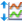
\includegraphics[width=4mm]{../src/edu/cornell/dendro/corina_resources/Icons/22x22/spreadvertically.png} & Spread the series evening up the vertical axis \\
 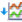
\includegraphics[width=4mm]{../src/edu/cornell/dendro/corina_resources/Icons/22x22/squeezevertically.png} & Set the baselines of all the series to zero \\
 
\includegraphics[width=4mm]{../src/edu/cornell/dendro/corina_resources/Icons/22x22/fitcharthoriz.png} & Resize graph to fit horizontally \\
 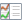
\includegraphics[width=4mm]{../src/edu/cornell/dendro/corina_resources/Icons/22x22/legend.png} & Toggle show/hide the legend\\
\end{tabular*}
\end{center}

There are also a number of keyboard shortcuts that you might find useful:

\begin{description*}
 \item[Tab] : Cycles through each graph component
 \item[Ctrl+W] : Increase vertical scale
 \item[Ctrl+S] : Decrease vertical scale
 \item[Ctrl+A] : Increase horizontal scale
 \item[Ctrl+D] : Decrease horizontal scale
 \item[Up arrow] : Moves selected graph up by 10 units
 \item[Down arrow] : Moves selected graph down by 10 units
 \item[+] : Moves selected graph up by 1 unit
 \item[-] : Moves selected graph down by 1 unit
 \item[HOME] : Scroll to first year of series
 \item[END] : Scroll to last year of series
 \item[PAGE UP] : Scroll left by one page width
 \item[PAGE DOWN] : Scroll right by one page width
 \item[SPACE] : Sets horizontal origin of all graphs to the same value 
\end{description*}

\section{Exporting graphs}

To export your graphs for use in reports you can go to \menutwo{File}{Export plot as PDF file}, or \menutwo{File}{Export plot as PNG file}.  This presents you with a dialog for setting the colors, labels and size of the exported image.  This functionality is due for an overhaul in the future to provide more flexible support for publication quality graphics.  
